% Chapter Template

\chapter{Petri net representation for subnets and hiding support. PNML} % Main chapter title

\label{Petri net representation for subnets and hiding support. PNML} % Change X to a consecutive number; for referencing this chapter elsewhere, use \ref{Chapter3}

\lhead{Chapter . \emph{Petri net representation for subnets and hiding support. PNML}} % Change X to a consecutive number; this is for the header on each page - perhaps a shortened title

%----------------------------------------------------------------------------------------
%       SECTION 1
%----------------------------------------------------------------------------------------
\section{Introduction}

Once explained how to split a net in several subnets, the next step is to define a way to hide one or more of those subnets.

 There is not literature about this
topic. Because of that I have to do a previous work about Petri net representation.
First of all  a way to represent subnet must be defined. Depending on the selected representation, the way to occult subnets may
be different or even impossible.

\section{Petri net representations}
There are four standard ways to represent Petri nets. Each one of them have their
properties, advantages and disadvantages. But I want to select one that I am able to represent any kind of Petri net, its subnets and allow to hide information without erasing it. 

\subsection{Graphic representation}

This is the clearest and extended way to represent Petri nets. It has a
very important advantage and it is that a picture is worth a thousand words.


Subnets can be defined simply drawing a vertical line. The right part is
one subnet and the left part is other subnet. Places and transitions
can be moved from one location to another depending on the subnet they are
situated. This is only an example. Other way would be to use colors for the
nodes (same color indicates same subnet) or use rectangles, etc.

\begin{example}[Graphic representation of a hidden subnet]
\label{ej:graphic_representation_hidden_subnet}
Let's take the following Petri net.


\[
\includegraphics[width=0.3\textwidth]{Figures/EleccionSubredZonasInfluencia_2.eps}
\]



I want to occult the part marked with an H, so the result is this graphic

\[
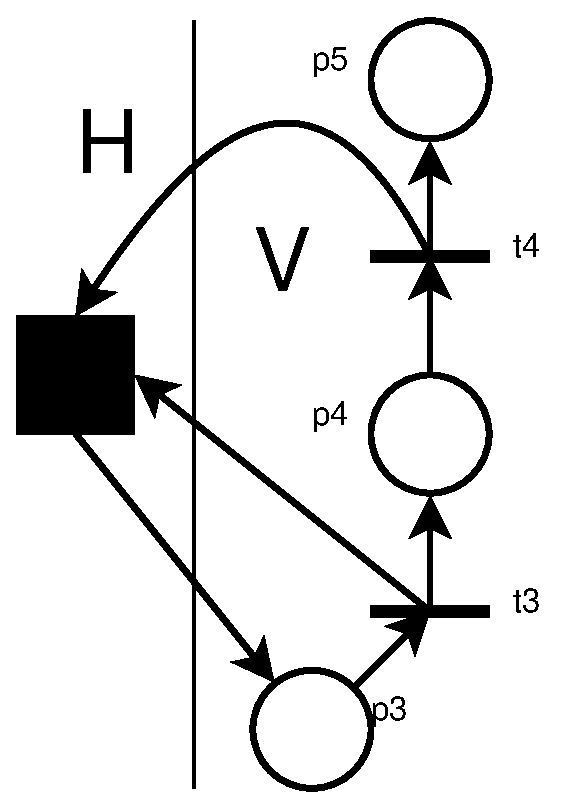
\includegraphics[width=0.25\textwidth]{Figures/OcultacionSubred_1.eps}
\]

And now, how can I maintain the H subnet information on the black box?
If I want to distribute  this Petri net I should send something more to that
people I want to access the hidden subnet. I have not found a way to embed
that information in the graphic so that some people can access it but other
people can't.
\end{example}

So this representation is useful in order to show at one sight the Petri
net structure, but I can't choose it  for my goals.
I have not been able to discover a way to show some people the hidden
information (the hidden subnet). However I will continue using it where a clear idea of the Petri structure
if necessary.

\subsection{Matrix representation}
This representation is very useful to study properties and evolution of a
Petri net, independently of its graphic representation.
As we have seen before (in chapter \ref{Chapter3}), we can reorder rows and columns and define subnets
in the matrix.
\begin{example}[Matrix representation of a hidden subnet]
\label{ej:matrix_representation_hidden_subnet}
This is the matrix representation of the Petri net in the previous example
\ref{ej:graphic_representation_hidden_subnet}.
\[
\kbordermatrix{
   & t_1 & t_2 & t_3 & t_4\\
p_1& -1 &  1  &  0  &  1 \\
p_2&  1 & -1  &  1  &  0 \\
p_3&  0 &  1  & -1  &  0 \\
p_4&  0 &  0  &  1  & -1 \\
p_5&  0 &  0  &  0  &  1 \\
}
\]

As we can see before,  If I occult the part marked with an H, so the result is:
\[
\kbordermatrix{
   & t_1 &  t_2 & \vline &t_3 & t_4\\
p_1& \rule{0.15in}{0.15in} & \rule{0.15in}{0.15in}    & \vline &  0  &  1 \\
p_2& \rule{0.15in}{0.15in} & \rule{0.15in}{0.15in}   & \vline &  1  &  0 \\
\hline
p_3&  0 &  1  & \vline & -1  &  0 \\
p_4&  0 &  0  & \vline &  1  & -1 \\
p_5&  0 &  0  & \vline &  0  &  1 \\
}
\]

or this other one, grouping the places and transitions of the hidden subnet as seen in chapter \ref{Chapter3}
\[
\kbordermatrix{
   &  _ & \vline &t_3 & t_4\\
p_2 & \rule{0.15in}{0.15in}   & \vline &  1  &  1 \\
\hline
p_3&  1  & \vline & -1  &  0 \\
p_4&  0  & \vline &  1  & -1 \\
p_5&  0  & \vline &  0  &  1 \\
}
\]


And now I have the same problems as in graphic mode: how can I keep  information
in the black box?
\end{example}

With this representation it is possible to study properties and it may be really important
as a complement to graphic mode. With both representations together, everyone has a clear idea of the Petri net structure and properties.  But I haven't
found a way to store information inside the black box. 

\subsection{Equation representation}
The third representation way for Petri nets is the equation representation.
Basically, transitions are selected and, for each one, the tokens of the places
connected to that transition are modified. This is very useful to compute
the evolution of a Petri net, choosing the transition fired.

However it is difficult to find a way for representing subnets with this
notation. And, of course, if a subnet cannot be represented, it cannot be
hidden. 

\begin{example}[Equation representation of a hidden subnet]
\label{ej:equation_representation_hidden_subnet}
Let's take again the Petri net from the previous examples \ref{ej:graphic_representation_hidden_subnet}.
This is It's equation representation:

\begin{scriptsize}
\begin{alltt}
if (p1>0) then
        p1 <- p1 - 1
        p2 <- p2 + 1
if (p2>0) then
        p2 <- p2 - 1
        p1 <- p1 + 1
        p3 <- p3 + 1
if (p3>0) then
        p3 <- p3 - 1
        p2 <- p2 + 1
        p4 <- p4 + 1
if (p4>0) then
        p4 <- p4 - 1
        p1 <- p1 + 1
        p5 <- p5 + 1
\end{alltt}
\end{scriptsize}

As we can see, we should hide several lines. In particular all that includes
places $p_1$ and $p_2$, resulting something like this (strikethrough text
would be part of the subnet):

\begin{scriptsize}
\begin{alltt}
\xout{if (p1>0) then}
        \xout{p1 <- p1 - 1}
        \xout{p2 <- p2 + 1}
\xout{if (p2>0) then}
        \xout{p2 <- p2 - 1}
        \xout{p1 <- p1 + 1}
        p3 <- p3 + 1
if (p3>0) then
        p3 <- p3 - 1
        \xout{p2 <- p2 + 1}
        p4 <- p4 + 1
if (p4>0) then
        p4 <- p4 - 1
        \xout{p1 <- p1 + 1}
        p5 <- p5 + 1
\end{alltt}
\end{scriptsize}

This is probably the strangest way to represent Petri nets and it is difficult
to define subnets over it.

\end{example}


I have tried to think about these ways of representation but, in my opinion, no one of them is suitable enough to represent subnets in a clear way than can be occulted. Because of that I have chosen the fourth representation, which is PNML, and that is explained in the next section. 

%----------------------------------------------------------------------------------------
%       SECTION 2
%----------------------------------------------------------------------------------------
\section{PNML. Petri Net Marked Language}

As I have explain in the Literature review in the chapter \ref{Chapter:LiteratureReview},
 PNML is a way to represent Petri nets as xml content.

The advantages over the other three representation ways described before
are clear. By one side, XML is a widely extended format to represent almost
everything. And not only that. XML is a robust technology free of errors
and it is really flexible. Its flexibility come from you can add any kind
of labels and functionality with a very little amount of work. Its robustness come from the strict
specification of the schemas declared to define completely the XML files    
that support. Once
the schema is defined, the XML files have a no way to get out of this definition,
so we can know if a XML file is correct given its schema. And this is not all. If you have an XML file, you can extract information to and complete it to create a schema for that file.  



Originally, with basic Petri nets, the structure of a Petri net was fully provided.
The only thing that is not supported in comparison with graphic mode is the graphical appearance of Petri nets: the position of nodes and
transitions was not
important, but with the arrival of High level Petri nets and Petri nets design
software, it is necessary to store this kind of information.

In this work, I am going to study only basic Petri nets, but
that concept and the method is easily exportable to other kind of nets, such as Symmetric nets and High Level Petri nets (that are representable in PNML
format too.)

\subsection{Scope}
The scope of this work in this section is basically bounded by the original
and basic Petri nets, that is:
\begin{itemize}
\item there are places, transitions and arcs between them
\item places can have tokens on them (but this does not have influence in
the hidding process)
\item transitions can be fired, but there is only one type of transition
(not messages, not time, etc.)
\end{itemize}

Furthermore, I am going to explain several concepts for a specific graphical
design of the Petri net (that will not influence the process either).

There are other options such as specific information for the design tool
that I am not going to discuss because the tools have no interest in this work 

\subsection{Description}
Petri Net Marked Language is an xml language created to represent Petri Nets. With this language we can take a Petri Net and store it into an xml file without loss of information.

One of the best properties of PNML is that, as it is an xml based schema,
it can be extended with more functionality extending the grammar.
Virtually, any extension over Petri nets can be translated into PNML in a logical and natural way.
Moreover, this extension is defined by Petri net type definition \cite{PNML-Billington2003483,PNML-iso/iec-15909-2:2011}.
 

In this case PNML hasn't got a way to represent subnets. There is something named \texttt{\textless page\textgreater}\ 
that is used to represent several nets in the same PNML file. But, by default,
a node inside a page cannot connect with a node of other page. So it cannot
be used as "subnets". So I am going to extend the language in order to get several goals:
\begin{enumerate}
\item Represent subnets of a Petri Net.
\item Include input and output interfaces for every subnet.
\end{itemize}

As we can think, definition of several subnets of a Petri net is possible
and the connection over them are always through their respective interfaces.

\subsection{PNML grammar}

As PNML is an xml based language it has to be described by an schema that define the creation rules of the PNML representation of a Petri net.

The grammar is defined since 2009 and updated until
2012, which is the most recent revision.
I am not going to do and extensive explanation of all the possibilities
of the grammar, but the most important. As we can see later, anything we think is useful can be added to the process with little effort.
So I am going to study only the most basic elements of a Petri net. The rest of the element can be attached later with facility. 

\subsubsection{PNML basics}

In this section I am going to explain several characteristics of PNML files.
With these explanations it is going to be easier the understanding of PNML
structure.

First of all, as PNML files are xml files, there several things to know:

\begin{enumerate}
\item 
  A xml file normally starts with a line defining some characteristics of
  the file, like the version and the encoding type. It has an aspect like
  this\footnote{For clarity, in the following examples, this line can be deleted.}: 

\begin{lstlisting}
<?xml version="1.0" encoding="utf-8"?>
\end{lstlisting}
  
 
\item
  A root node must exist.
  In this case, the root node is \texttt{\textless pnml\textgreater}.
  So every PNML files has to start with the tag \texttt{\textless pnml\textgreater}\   and end with the tag \texttt{\textless/pnml\textgreater}.
Below this tag, there is a new tag \texttt{\textless net\textgreater}\ that can contain
  \begin{itemize}
  \item Type: the type of the Petri net as an attribute. In this case, as
    I  am going to study only Place/Transition nets, it will  be \texttt{ptnet}
  \item Name of the net: New tag \texttt{\textless name\textgreater\textless text\textgreater...\textless/text\textgreater\textless/name\textgreater}
  \item Pages: one page is an invention to store several Petri nets inside
  an unique PNML file, but usually there is only one page for file. It is
  nested inside a \texttt{\textless page\textgreater}\ tag.
  \end{itemize}
  \item
  Each element in PNML has to have a unique id inside the net to be identified
unambiguously. So there cannot
  be two elements with the same id.
\end{enumerate}

 

With this three observations, we can have an idea about how a PNML file
is structured:  

 
\begin{lstlisting}[label=pnml_net_page,caption=Example of general PNML file]
<?xml version="1.0" encoding="utf-8"?>
<pnml>
  <net id="myNet" type="http://www.pnml.org/version-2009/grammar/ptnet">
    <name>
      <text> My new net </text>
    </name>
    <page id="page1">
      .......
    </page>
  </net>
</pnml>
\end{lstlisting}

Once this structure is defined, I am going to explain the next stage, that
is the most important one in this work. 

\subsubsection{Places, transitions and arcs in PNML}

As Petri nets has three main elements, places, transitions
and arcs, and PNML has them too. These three elements have several things in common in an PNML file:
\begin{itemize}
  \item They are all nested in a page tag


  \item Places and transitions (not arcs) can contain a tag \texttt{\textless name\textgreater}\ with its name. This tag has been defined before for the name of the net. It
can store information about the text of the name and the graphical position
of this label in this way:
\begin{lstlisting}
<name>
  <text> Element Name </text>
  <graphics>
    <offset x="22" y="-10"/>
  </graphics>
</name>
\end{lstlisting}
   \item They can contain a tag \texttt{\textless graphics\textgreater}\ with information about its position and dimension:
\begin{lstlisting}
<graphics>
  <position x="100" y="200"/>
  <dimension x="40" y="40"/>
</graphics>
\end{lstlisting}
\end{itemize}


These are the common properties of places, transitions and arcs. Now let's
go on the particular characteristics of each one of them.

Places are represented with the tag \texttt{\textless place\textgreater}\ and the can have a marking with the label \texttt{\textless initialMarking\textgreater}.
Here we have an example of a place with two tokens in PNML: 

\begin{lstlisting}[label=pmnl_place,caption=PNML representation
for places]
<place id="p1">
  <name>
    <text> Place number one </text>
    <graphics>
      <offset x="130" y="130"/>
    </graphics>
  </name>
  <graphics>
    <position x="130" y="90"/>
    <dimension x="40" y="40"/>
  </graphics>
  <initialMarking>
    <text> 2 </text>
  </initialMarking>
</place>
\end{lstlisting}

Transitions are represented with the tag \texttt{\textless transition\textgreater}.
This is an example of a transition in PNML: 

\begin{lstlisting}[label=pmnl_transition,caption=PNML representation
for transitions]
<transition id="t1">
  <name>
    <text> Transition number one </text>
    <graphics>
      <offset x="270" y="140"/>
    </graphics>
  </name>
  <graphics>
    <position x="270" y="100"/>
    <dimension x="40" y="40"/>
  </graphics>
</transition>
\end{lstlisting}

Arcs are represented with the tag \texttt{\textless arc\textgreater}. Arc
have to have a source and a target, which are defined by the attributes \texttt{source} and \texttt{target} that have to point to a transition and a place, identified
by their id. Furthermore, the arc weight can be fixed by the \textless inscription\textgreater\
 tag.
If the weight is one, the tag inscription is not necessary because this is
the default value. This is an example of the arc with weight 3 that connects the place and the
transition of the previous examples in PNML: 

\begin{lstlisting}[label=pmnl_arc,caption=PNML representation
for arcs]
<arc id="a1" source="p1" target="t1">
  <inscription> 3 </inscription>
</arc>
\end{lstlisting}

\newpage
If we take the last examples all together, we can represent the following Petri net:

\[
\includegraphics[width=0.25\textwidth]{Figures/PNML-RdPBasicaCompleta.eps}
\]

\begin{lstlisting}[label=pmnl_complete_representation,caption=Complete PNML representation
for a basic Petri net]
<?xml version="1.0" encoding="utf-8"?>
<pnml>
  <net id="myNet" type="http://www.pnml.org/version-2009/grammar/ptnet">
    <name>
      <text> My new net </text>
    </name>
    <page id="page1">
      <place id="p1">
        <name>
          <text> Place number one </text>
          <graphics>
            <offset x="130" y="130"/>
          </graphics>
        </name>
        <graphics>
          <position x="130" y="90"/>
          <dimension x="40" y="40"/>
        </graphics>
        <initialMarking>
          <text> 2 </text>
        </initialMarking>
      </place>
      <transition id="t1">
        <name>
          <text> Transition number one </text>
          <graphics>
            <offset x="270" y="140"/>
          </graphics>
        </name>
        <graphics>
          <position x="270" y="100"/>
          <dimension x="40" y="40"/>
        </graphics>
      </transition>
      <arc id="a1" source="p1" target="t1">
        <inscription> 3 </inscription>
      </arc>
    </page>
  </net>
</pnml>
\end{lstlisting}

For clarity, I am going to obviate several options. I am not going to put the graphic information and the names, but the id. So this last example is as follows:

\[
\includegraphics[width=0.1\textwidth]{Figures/PNML-RdPBasica.eps}
\]

\begin{lstlisting}[label=pmnl_basic_representation,caption=Basic PNML representation
for a basic Petri net]
<?xml version="1.0" encoding="utf-8"?>
<pnml>
  <net id="myNet" type="http://www.pnml.org/version-2009/grammar/ptnet">
    <page id="page1">
      <place id="p1">
        <initialMarking>
          <text> 2 </text>
        </initialMarking>
      </place>
      <transition id="t1"/>
      <arc id="a1" source="p1" target="t1">
        <inscription> 3 </inscription>
      </arc>
    </page>
  </net>
</pnml>
\end{lstlisting}


I think that this last listing is clear enough to understand the rest of
the process. But not only that. For even more clarity, the tags \texttt{\textless ?xml\textgreater}, \texttt{\textless pnml\textgreater}, \texttt{\textless net\textgreater}\ and \texttt{\textless page\textgreater} are going to be obviated
too. So in many of the later examples they will not be present. Applying
this criterium, the listing \ref{pmnl_basic_representation} change to:

\begin{lstlisting}[label=pmnl_simplified_representation,caption=Simplified PNML representation
for a basic Petri net]
<place id="p1">
  <initialMarking>
    <text> 2 </text>
 </initialMarking>
</place>
<transition id="t1"/>
<arc id="a1" source="p1" target="t1">
  <inscription> 3 </inscription>
</arc>
\end{lstlisting}








\subsection{PNML examples}

In this section I will present several examples of  Petri nets represented with PNML. This examples are extracted directly form \url{www.pnml.org}.
These examples will be processed later in order to hide parts of them.

As first example, we have the Dining Philosophers...

//TODO terminar 

\subsection{PNML extension for representing subnets}


 In this section I am going to define new tags and structures in PNML. At this point, I have developed all the necessary to extend PNML in order
to represent subnets.

Let's take the following simple Petri net that will serve us to explain
the method to achieve a subnet representation and the PNML extension associated
to it:

\[
\includegraphics[width=0.40\textwidth]{Figures/PNML-RdPSubred.eps}
\]

The PNML code for this net is:

\begin{lstlisting}
<place id="p1"/>
<place id="p2"/>
<place id="p3"/>
<transition id="t1"/>
<transition id="t2"/>
<transition id="t3"/>
<arc id="a1" source="p1" target="t1">
  <inscription>
    <text> 3 </text>
  </inscription>
</arc>
<arc id="a2" source="t1" target="p2"/>
<arc id="a3" source="t1" target="p3"/>
<arc id="a4" source="p3" target="t2">
  <inscription>
    <text>2</text>
  </inscription>
</arc>
<arc id="a5" source="t3" target="p3"/>
<arc id="a6" source="p2" target="t3"/>
<arc id="a7" source="t2" target="p1"/>
\end{lstlisting}

I want the ellipse region to be a subnet, so I have to specify a subnet with the elements inside the ellipse.



The first step is to define a new tag \texttt{\textless subnet\textgreater}. This tag will have an id, as the rest of PNML elements. And now we proceed
in this way:

\begin{enumerate}
\item The places and transitions inside the subnet are moved into the \textless subnet\textgreater\ tag
\item The arcs joining subnet elements will be included inside the tag
\item The arcs entering or leaving the subnet will be copied inside the tag.
This mean that there are arcs duplicated inside and outside the tag
\end{enumerate}


If we apply these rules to the example:

\begin{enumerate}
\item $p2$, $p3$ and $t3$ are moved into the tag \texttt{\textless subnet\textgreater}
\item $a5$ and $a6$ are put inside the tag
\item $a2$, $a3$ and $a4$ are copied inside the tag
\end{enumerate}

and we have this other PNML extended code: 

\begin{lstlisting}
<subnet id="sn1">
  <place id="p2"/>
  <place id="p3"/>
  <transition id="t3"/>
  <arc id="a2" source="t1" target="p2"/>
  <arc id="a3" source="t1" target="p3"/>
  <arc id="a4" source="p3" target="t2">
    <inscription>
      <text> 2 </text>
    </inscription>
  </arc>
  <arc id="a5" source="t3" target="p3"/>
  <arc id="a6" source="p2" target="t3"/>
</subnet>
<place id="p1"/>
<transition id="t1"/>
<transition id="t2"/>
<arc id="a1" source="p1" target="t1">
  <inscription>
    <text> 3 </text>
  </inscription>
</arc>
<arc id="a2" source="t1" target="p2"/>
<arc id="a3" source="t1" target="p3"/>
<arc id="a4" source="p3" target="t2">
  <inscription>
    <text> 2 </text>
  </inscription>
</arc>
<arc id="a7" source="t2" target="p1"/>
\end{lstlisting}

Now this is one of the most important moment in this work: I will separate the inside
and the outside of the subnet completely. Taking advantage of the process described in chapter \ref{Chapter3}, I have to extract the front-end from this subnet.

In this case I have two igp (input gate to a place) and an ogt (output gate to a transition). This graphic illustrates the interface associated:

\[
\includegraphics[width=0.60\textwidth]{Figures/PNML-InterfazSubredEjemplo1.eps}
\]

And this is the complete net including the subnet and its front-end

\[
\includegraphics[width=0.60\textwidth]{Figures/PNML-SubredEjemplo1.eps}
\]
 
And now that I have the graphic, how can I represent it in PNML? To answer
this question I will define four new tags: \texttt{\textless interface\textgreater},
\texttt{\textless gate\textgreater}, \textless inscription\textgreater\ and \texttt{\textless content\textgreater}. Let's explain them.

As its name says, \texttt{\textless interface\textgreater}\ is
the tag name for encapsulate the front-end. This tag has no attributes (only
the id, of course)
but
it has embedded the gates inside of it. This gates are represented by \texttt{\textless gate\textgreater}. This tag has two new attributes: \texttt{action} and \texttt{type}.
These two attributes have information about the gates. The attribute \texttt{action}
can take two different values: \texttt{input} and \texttt{output}. It indicates
whether the gate is an input gate or an output gate. The other attribute,
\texttt{type}, can take other two values: \texttt{place} and \texttt{transition}.
As arcs have weight, gates have it too. For being in accordance, I define
the tag \texttt{\textless inscription\textgreater}\ embedded in the tag \texttt{\textless gate\textgreater}. It has the weight of the arc associated.\ 

There is one other tag \texttt{\textless content\textgreater}\ that
probably at this moment seems useless, but it is necessary for the rest of the process, as we will see in the next chapter. So I am going to introduce it now. This tag is used to encapsulate the rest of the subnet outside the interface. That is, \texttt{\textless subnet\textgreater}\ has two children:
\texttt{\textless interface\textgreater}\ and \texttt{\textless content\textgreater},
that have the input/output gates and the rest of the elements, respectively.

Applying this definition to the example, we will have this code

\begin{lstlisting}
<subnet id="sn1">
  <interface id="sn1-interface">
    <gate id="igp1" action="input" type="place"/>
    <gate id="igp2" action="input" type="place"/>
    <gate id="ogt1" action="output" type="transition">
      <inscription>
        <text> 2 </text>
      </inscription>
    </gate>
  </interface>
  <content id="sn1-content">
    <place id="p2"/>
    <place id="p3"/>
    <transition id="t3"/>
    <arc id="a2" source="t1" target="p2"/>
    <arc id="a3" source="t1" target="p3"/>
    <arc id="a4" source="p3" target="t2">
      <inscription>
        <text> 2 </text>
      </inscription>
    </arc>
    <arc id="a5" source="t3" target="p3"/>
    <arc id="a6" source="p2" target="t3"/>
  </content>
</subnet>
<place id="p1"/>
<transition id="t1"/>
<transition id="t2"/>
<arc id="a1" source="p1" target="t1">
  <inscription>
    <text> 3 </text>
  </inscription>
</arc>
<arc id="a2" source="t1" target="p2"/>
<arc id="a3" source="t1" target="p3"/>
<arc id="a4" source="p3" target="t2">
  <inscription>
    <text> 2 </text>
  </inscription>
</arc>
<arc id="a7" source="t2" target="p1"/>
\end{lstlisting}

At this moment I have to do only one thing more. The last step is to modify
the arcs that are repeated inside and outside the net changing their source or target, depending on where is it:

\begin{itemize}
\item If the arc is \textbf{entering} the subnet
  \begin{itemize}
  \item For the \texttt{\textless arc\textgreater} tag inside the tag \texttt{\textless subnet\textgreater}, the \textbf{source} attribute of the arc is changed by the \textbf{input} gate associated
  \item For the \texttt{\textless arc\textgreater} tag outside the tag \texttt{\textless subnet\textgreater}, the \textbf{target} attribute of the arc is changed by the \textbf{output} gate associated
  \end{itemize}
\item If the arc is \textbf{leaving} the subnet
  \begin{itemize}
  \item For the \texttt{\textless arc\textgreater} tag inside the tag \texttt{\textless subnet\textgreater}, the \textbf{target} attribute of the arc is changed by the \textbf{input} gate associated
  \item For the \texttt{\textless arc\textgreater} tag outside the tag \texttt{\textless subnet\textgreater}, the \textbf{source} attribute of the arc is changed by the \textbf{output} gate associated
  \end{itemize}
\end{itemize}

Applying again this rule to the example we have the definitive code for this
Petri net:

\begin{lstlisting}
<subnet id="sn1">
  <interface id="sn1-interface">
    <gate id="igp1" action="input" type="place"/>
    <gate id="igp2" action="input" type="place"/>
    <gate id="ogt1" action="output" type="transition">
      <inscription>
        <text> 2 </text>
      </inscription>
    </gate>
  </interface>
  <content id="sn1-content">
    <place id="p2"/>
    <place id="p3"/>
    <transition id="t3"/>
    <arc id="a2" source="igp2" target="p2"/>
    <arc id="a3" source="igp1" target="p3"/>
    <arc id="a4" source="p3" target="ogt1">
      <inscription>
        <text> 2 </text>
      </inscription>
    </arc>
    <arc id="a5" source="t3" target="p3"/>
    <arc id="a6" source="p2" target="t3"/>
  </content>
</subnet>
<place id="p1"/>
<transition id="t1"/>
<transition id="t2"/>
<arc id="a1" source="p1" target="t1">
  <inscription>
    <text> 3 </text>
  </inscription>
</arc>
<arc id="a2" source="t1" target="igp2"/>
<arc id="a3" source="t1" target="igp1"/>
<arc id="a4" source="ogt1" target="t2">
  <inscription>
    <text> 2 </text>
  </inscription>
</arc>
<arc id="a7" source="t2" target="p1"/>
\end{lstlisting}

Once this is done, the only way to enter or leave the subnet is crossing
the front-end. 







\section{Conclusions}


